\documentclass[conference]{IEEEtran}
\IEEEoverridecommandlockouts
% The preceding line is only needed to identify funding in the first footnote. If that is unneeded, please comment it out.
%Template version as of 6/27/2024

\usepackage{cite}
\usepackage{amsmath,amssymb,amsfonts}
\usepackage{algorithmic}
\usepackage{graphicx}
\usepackage{textcomp}
\usepackage{xcolor}
\usepackage{listings}
\usepackage[top=0.75in, bottom=1.05in, left=0.6in, right=0.6in]{geometry}
\lstset{breaklines=true, basicstyle=\footnotesize\ttfamily}
\def\BibTeX{{\rm B\kern-.05em{\sc i\kern-.025em b}\kern-.08em
    T\kern-.1667em\lower.7ex\hbox{E}\kern-.125emX}}

\begin{document}

\title{Using Graph Cycle Detection to Reveal Suspicious Ethereum Token Transfer Behaviour
\thanks{Special thanks to Horizon Globex Ltd. CEO Brian Collins, in conjunction with Lero, the Irish software engineering research center for supporting this work.}
}

\author{\IEEEauthorblockN{Dr. Andrew Le Gear}
\IEEEauthorblockA{\textit{Horizon Globex Ltd.} \\
Limerick, Ireland \\
andrew.legear@horizon-globex.ie}
\and
\IEEEauthorblockN{Dr. Farshad Ghassemi Toosi}
\IEEEauthorblockA{\textit{Munster Technological University} \\
Cork, Ireland \\
farshad.toosi@mtu.ie}
\and
\IEEEauthorblockN{Dr. Ashish Rajendra Sai}
\IEEEauthorblockA{\textit{University of Maastrict} \\
Maastrict, The Netherlands \\
ashish.sai@maastrichtuniversity.nl}
\and
\IEEEauthorblockN{Tawny Whatmore}
\IEEEauthorblockA{\textit{Horizon Globex Ltd.} \\
Limerick, Ireland \\
tawny.whatmore@horizon-globex.com}
\and 
\IEEEauthorblockN{Dr. Jim Buckley}
\IEEEauthorblockA{\textit{Lero - University of Limerick} \\
Limerick, Ireland \\
jim.buckley@ul.ie}
}

\maketitle

\begin{abstract}
In the unregulated world of Initial Coin Offerings (ICOs),  hiding malicious trading is all too easy in a large-scale set of transactions.  This paper uses a graph-based representation of the blockchain to identify a topology that reveals suspicious intent to manipulate the perceived value of those offerings. As the computational complexity of identifying this topology could be prohibitive for unfiltered data-sets, this work derives metrics indicative of the topology. Using these explicitly-defined metrics and a past degradation of service on the Ethereum network originating with the iFishYunYu token, we show how this approach can reveal it to have been a deliberate attack, rather than simply an unprecedentedly highly-traded token. The formalization of this approach in the paper will allow detection of other such ``pump-and-dump'' attacks in the future.
\end{abstract}

\begin{IEEEkeywords}
Blockchain, Ethereum, Smart Contract, Reverse Engineering, Graph Analysis
\end{IEEEkeywords}



\section{Introduction}

Reports suggest that cryptocurrencies have grown to an over \$300 billion market capitalization \cite{griffin2018tethered}. However, financial regulations are only beginning to play catch-up in this, largely-unregulated financial world and this leaves cryptocurrencies vulnerable to manipulation. For example, the Bitcoin ecosystem has been frequently attacked for financial gain \cite{griffin2018tethered}, \cite{Ganda12018PriceManip}.

The research presented here focuses on detection of such attacks. In this paper we focus on ``pump-and-dump'' attacks \cite{jiang2005market} as an initial exemplar. A ``Pump-and-Dump'' market manipulation can be defined as a scenario where a deceiver first buys a stock and then enlists a promoter to tout the stock by spreading positive messages, thereby manipulating the share price and selling the stock at a profit \cite{siering2019economics}.  In this paper's scenario we look to equivalent pump-and-dump schemes orchestrated on the blockchain.  This is where a token's value is artificially inflated through the dissemination of false information on/impressions of the token. For example, the token's price can be artificially inflated by creating a ``rush'' on the token, where lots of different wallets purchase the tokens at an artificial price (the ``pump'') but where these wallets ultimately get their currency from the same (or a few) origins. Unsuspecting traders witnessing what on the surface would be a volume signal to purchase the tokens at the manipulated price, enter the market.  The manipulator then exits his position at the higher price (the ``dump''). In detecting such attacks as they happen, this research offers alerts to potential investors as to the danger of investing in the offerings.

Thus, this paper makes the following contributions:

\begin{itemize}
    \item A novel analysis technique, embodied as an explicitly defined metric, based on observations of the graph-structure of indicative blockchain transactions, for revealing suspicious pump-and-dump trading behaviour surrounding ERC-20 \cite{vogelstellerbuterin} traded token contracts.
    \item An illustration and evaluation of the graph topology/metric using a real-world case study of the iFishYunYu attack on the Ethereum network.
    \item A threshold for the metric, calibrated to the results of the analysis of the iFishYunYu contract.
\end{itemize}

\section{Related Work} \label{relatedwork}

\subsection{Graph Cycle Detection} \label{graphcycles}
The analysis technique proposed here is based on a variation of standard cycle detection approaches from graph theory. Our internal model of the blockchain transaction-set is represented as an undirected graph. The nature of the data means that the graph is not \emph{strongly connected}\footnote{There is always a path from one node to another if the graph is \emph{strongly connected}.} or \emph{simple}\footnote{There are no cycles in the graph if the graph is \emph{simple}}. To detect the presence of a cycle in a graph you perform a \emph{depth first search} that tracks visited nodes and a stack representing the current traversal.  When a visited node in your stack repeats you have identified a cycle \cite{cormen2009introduction}.

The running time for a typical cycle detection algorithm\cite{cormen2009introduction}, where all cycles must be detected, is $\Theta(V+E)$.  This is an impressive running time.  Unfortunately, for our technique we must be able to enumerate all the distinct cycle paths, including the paths of smaller cycles whose sub-paths are included in larger cycles which results in the execution running into polynomial times. Johnson in \cite{johnson1975finding}, for example, proposes listing the exhaustive set of cycle paths in a directed graph resulting in a running time of $\Theta((V + E)(c + 1))$, where $c$ is the number of cycles. Proposed refinements to the algorithm are worthy improvements but never escape the burden of polynomial time.  Notably we have Paton \cite{paton1969algorithm} and Birmel et. al. \cite{birmele2013optimal} providing implementations for undirected graphs, which is particularly applicable to us.   Our traversal, as described in Section \ref{graphtraversal}, suffers from the polynomial performance alluded to here.  We make two important decisions in order to time limit our traversal and make the technique more real-world applicable:

\begin{enumerate}
    \item We choose a specific start point for the traversal - i.e. the graph node representing the ERC-20 we wish to analyze.  
    \item We choose the specific cycle lengths that we are interested in. 
\end{enumerate}

\subsection{Software Reverse Engineering}\label{RevEng}
Our approach to blockchain analysis draws upon the field of \emph{software reverse engineering}.  Software reverse engineering refers to moving up the abstraction hierarchy from lower level development artifacts like code to higher level abstractions from earlier in the development cycle like UML diagrams or architectural designs \cite{chikofsky1990reverse}. Program Dependency Graphs\cite{fan2012testing}, Module Dependency Graphs \cite{mamaghani2009clustering}, Object-oriented Dependency Graphs \cite{chen1997object}, and System Dependency Graphs \cite{sinha1999system} have all been widely used to analyze software. The dependencies that they graph almost always focus on first class language constructs exclusively. However, in some examples, these graphed constructs extend to file accesses \cite{moser1990data}, \cite{cleve2006data}, database calls \cite{liu2011extraction}, distributed systems dependencies \cite{holtzblatt1997design} and concurrency \cite{zhao1999multithreaded}. Graphs in this paper are used as our source model represents Ethereum transactions.  

A sizable proportion of the software reverse engineering space implements their techniques using graph representation as input.  As such, the research space provides a wealth of potentially useful techniques that could potentially be applied to blockchain analysis also \cite{kramer1996design} \cite{duenas1998architecture} \cite{fan2012testing} \cite{mamaghani2009clustering} \cite{chen1997object} \cite{lee2010study} \cite{holtzblatt1997design} \cite{willmor2004program}. 
For example, a simple depth-first-search to uncover transitive closure in source-model graphs is used in reverse engineering to signal mutually recursive routines in these source models \cite{cimitile1995software}.


\subsection{Ethereum and Smart Contracts}

Instrumental in enabling the proliferation of new use cases of distributed ledger technology is the ``Ethereum.'' blockchain \cite{dhillon2017unpacking}.  In one sense, Ethereum is a traditional cryptocurrency platform like Bitcoin, with it's native cryptocurrency Ether.  However, a transfer of Ether between parties is just one of an entire set of byte-code instructions supported by the Ethereum Virtual Machine (EVM). This full blown instruction set allows for complex programs to be run and store states in what are known as ``Smart Contracts.'' \cite{buterin2014next}  The higher-level programming language Solidity, allows for the definition of these Smart Contracts to be written and compiled to the EVM bytecode and subsequent deployment to the blockchain \cite{dannen2017introducing}.  

A common use case of smart contracts is to virtually model the ownership of an asset in much the same way as a share certificate represents ownership of a business issued from a stock exchange.  This is referred to as a ``token'' or ``coin.'' The Ethereum foundation define standards for how common smart contract use cases should be defined.  The common standard used to model token ownership is known as ``ERC-20'' \cite{vogelsteller2018erc} and it provides definitions for transfer of tokens and querying balances of minted and allocated tokens. %% At the time of writing this paper \footnote{August 2019} there were over 208,297 ERC-20 contracts deployed to Ethereum, the top 50 of which had a combined market capitalization of \$16.3 billion.  
Creating a new token and distributing it to investors in this fashion on the blockchain is known as an \emph{Initial Coin Offering}(ICO),  \emph{Token Generation Event}(TGE) or \emph{Security Token Offering}(STO).

\subsection{Blockchain Analysis}
The importance of being able to analyze and reverse engineer the content of the blockchain is beginning to be recognized. Attempts from several different research angles have begun to appear, albeit mostly examining the Bitcoin network.  

BlockSci \cite{kalodner2017blocksci}, for example, proposes an extraction flow similar to that proposed in this article, including internally represented transaction graph.  The queries examined however are more relational than graph-based.

Recent advancements in machine learning and Graph Neural Networks (GNNs) have significantly enhanced blockchain anomaly detection capabilities.
These methods excel at learning complex patterns and improving accuracy in identifying various illicit activities \cite{Chen2024Phishing, Harper2025STGNN, Gu2025Ensemble, Sultana2025GNN}.

In \cite{bragagnolo2018ethereum} a dedicated domain specific query language is proposed.  They propose their DSL as a basis for other research analysis projects on Ethereum, however for now it suffers from scalability limitations.

\cite{pinna2017petri} is a cross-domain application of Petri Nets to the blockchain.  They focus their analysis on single use wallets.

Very uniquely, \cite{spagnuolo2014bitiodine} scrapes several secondary sources of data, such as forums and groups, to match real world identities to the otherwise anonymous wallets of the blockchain.  Successful attempts at revealing identity on the blockchain can also be found in \cite{fleder2015bitcoin}. Notably they extract the Bitcoin blockchain to a graph representation. They apply a PageRank\cite{page1999pagerank} traversal, like that of popular search engines, to identify the most popular wallets in the network.

In a similar vein, the Monero blockchain  promotes its ability to hide the source of transactions, however \cite{kumar2017traceability} shows, with their technique, that they can break this anonymity in the vast majority of cases. 

We see an example of a traditional software reverse engineering approach using Eigen decomposition to reveal coordinated use of wallets when executing contracts on the Ethereum network in \cite{ghassemi2018reverse}. Also, \cite{moser2013inquiry} uses traditional reverse engineering techniques applied to to the Bitcoin blockchain for the purposes of Anti Money Laundering and Know Your Customer procedures mandated by law for banking and financial services.



\section{Using Graph Cycles to Reveal Suspicious Behaviour} \label{ourapproach}
%abstract overview followed by bullet points.  explain purpose and desired output first


In Figure \ref{fig:lifecycle} we summarize our analysis approach as follows:

\begin{enumerate}
    \item We host an instance of an Ethereum node connected to the Ethereum Frontier network \footnote{``Frontier'' is the name given to the production Ethereum network.}.  We use Parity's implementation, however any node that implements the Ethereum standard JSON-RPC protocol \cite{kalodner2017blocksci} can be swapped in place here.
    \item Using a small C\# Azure Function \cite{vijayakumar2018serverless} script we loop over the blockchain extracting the desired snapshot and writing output in graphSON \cite{tomaszuk2016rdf} format to a file.
    \item The graphSON file of our extract is imported into Apache Tinkerpop, a graph DB \cite{jouili2013empirical}, to allow us perform efficient graph traversal queries on the data.
    \item Applying a Gremlin query to the imported snapshot, we extract a sub-graph containing only the cycles detected and export the sub-graph to a graphML \cite{brandes2013graph} file.
    \item The extracted sub-graph is imported to a visualization tool - in this case we use Gephi \cite{bastian2009gephi} to visualize our graph.
    
\end{enumerate}

\begin{figure}
    \centering
    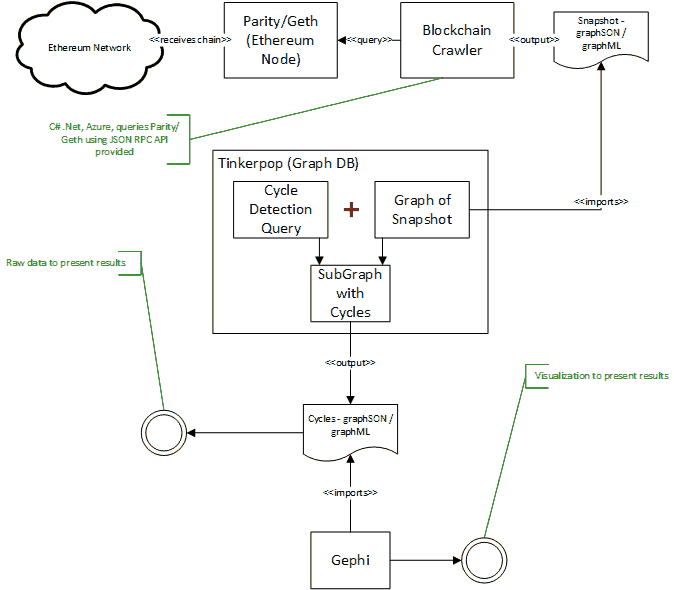
\includegraphics[width=0.8\columnwidth]{images/graph_analysis_lifecycle.png}
    \caption{Our Analysis Lifecycle}
    \label{fig:lifecycle}
\end{figure}

\subsection{Blockchain Extraction} \label{extraction}
At the time of writing there were 105,000,000 transactions on the Ethereum blockchain.  Without the purchase of dedicated hardware,  memory or the engineering of a sharded database infrastructure across a farm of machines,  it would be impractical to extract and model the entire blockchain in memory.  Fortunately,  the nature of our analysis approach allowed us to be very selective of the data we need.  Firstly, any blockchain data prior to the deployment of the contract under analysis can be ignored. Secondly, our approach should be targeted at a period of time where one suspects malicious activity.  For example,  an ERC-20 will usually have low volumes of activity until post-ICO, since the tokens are often not tradeable until the ICO closes. So focusing on post-ICO activity of the contract that exhibits high trading volumes would be prudent and further narrows the snapshot extracted.

\subsection{Graph Definition}\label{graphdefinition}
Our analysis approach relies on a blockchain snapshot modelled as an undirected cyclic graph. The vertices represent wallets or contracts on the blockchain and the edges represent transactions.  The edges express the transfer of value from the out vertex to the in vertex.  This could be a wallet transferring Ether to another wallet or contract,  or it could also be an ERC-20 contract transferring tokens to a wallet. However, unlike a wallet, whose actions are human initiated, a transfer of value from an ERC-20 contract cannot be initiated by the contract.  It can only be initiated by the wallet receiving tokens from the contract when that wallet invokes the ``transfer()'' method of the contract. As a result, even though the contract is transferring tokens from the contract to a wallet,  it appears as a transaction from the wallet to the contract on the blockchain. While this is perfectly legitimate, the ambiguous and sometimes dual flow of value is the primary motivation for modelling the transactions as undirected.  

\subsection{Graph Traversal}\label{graphtraversal}
% tinker pop query - break it down - relate to cycle detection section - summary of query language
We implement the extraction of a sub-graph of cycles from our blockchain snapshot using a graph traversal query language called Gremlin \cite{rodriguez2015gremlin}.  Gremlin is supported by several graph databases \cite{holzschuher2013performance}, but specifically in our implementation, we use Tinkerpop \cite{jouili2013empirical}.  The following is an annotated query that explains the extraction of the sub-graph in line with how we described our approach from previous sections (Note that the traversal in our approach must originate from a chosen ERC-20 contract vertex under analysis.  This focuses the query for the user and also improves performance significantly):

\begin{lstlisting}[basicstyle=\tiny]
   g.V() // Get the vertices connected on each end of the edge
   .has('account','hex',
      '0x98b4ca8bd52e4ed1f2
        8d3f30d9f567d1166c9483'
   ).as('a')   // select only the iFish contract vertex
   .bothE().bothV()   // Traverse the incoming and implied 
   // outgoing edges from iFish 
   .repeat( simplePath() // repeat edge traversal 
      // without repeated vertices
   ).times(2)   // repeat for a maximum of two further iterations
   .where(out().as('a')) // filter to the set of traversals where
      // the last outgoing vertex is a cycle back to the iFish node
   .bothE() // include the last edge to iFish 
      // so we have a complete graph in our output
   .dedup() // remove any duplicate traversals
   .subgraph('subg') // collate the traversals generated 
      // in a new sub-graph
   .cap('subg') // halt at an execution barrier until all threads
      // for each traversal completes
   .next() // output the complete sub-graph
    
\end{lstlisting}





Graph databases are particularly efficient at processing traversals of graph based data, especially where queries can be subdivided into independent sub problems.  For example, the depth first search that forms the basis of the cycle detection described in Section \ref{graphcycles} can easily be paralellized as combination of many traversals of smaller sub graphs \cite{cormen2009introduction}.  A common parallelization idiom to apply in this type of scenario is known as ``MapReduce'' \cite{dean2008mapreduce} and is supported by many graph databases \cite{navarro2014graphdb}.  Not only does it allow efficient parallelization of the problem through multi-threading,  but also  by distributing the solution of the traversal to an entire farm of commodity machines with the result aggregated and reported once complete.  This is exactly the type of deployment solution applied by organizations such as Facebook and LinkedIn when executing traversals of their billion-plus sized graph databases \cite{shimpi2012overview}.  Should we want to expand our analyses to larger snapshots of the blockchain in the future, this would be the optimal model to apply. 

\subsection{Reporting and Visualization}\label{visualisation}
The outputted graphML representation of the cycle sub-graph is certainly useful on its own. However, adding a visualization of the graph combined with a good layout algorithm can be very helpful in eliciting new insights into the data.  We use the free graph visualization tool Gephi\cite{bastian2009gephi} with the embedded visualization algorithm ``Force Atlas 2.'' Force Atlas 2 belongs to the family of force-directed algorithms that make use of connectivity between pairs of nodes in order to calculate attraction and/or repulsion forces. Force Atlas 2 is similar to the classical Fruchterman Rheingold \cite{Fruchterman:1991:GDF:137556.137557} algorithm. Force Atlas 2 is the optimized version of Force Atlas in Gephi that can handle large graphs with reasonable quality and better complexity ($\theta(Nlog(N)$)\cite{barnes}.


\subsection{A Pump-and-Dump Metric}
The visualization of the cycles around a token in a transaction graph, during a trading period, can make the presence of suspect behaviour intuitively apparent - and this is one goal of our technique; to provide non-technical users a means to reveal such fraudulent scenarios visually. However, to further corroborate our results, we also propose a separate metric, that does not rely on cycles, to arrive at the same conclusions quantitatively during our evaluation. To formalize this, we propose a simple metric that reflects the ``common-ancestor'' cycles observed in these transaction graphs. That is, the metric attempts to express the proportion of wallets that transfer value to the ERC-20 that also share a common ancestor at various different levels of indirection from that ERC-20.

We define the \emph{``Funding-Origin Indirection Metric''}, $\iota$, over $n$ levels of ancestors, given:

\begin{itemize}
    \item The number of wallets, $\psi$ , that transfer currency to the ERC-20 in question.
    \item The number of wallets $\tau$, that transfer currency to the ERC-20 in question, that share common ancestors at level $x$, but not below level $x$, where $n \geqslant x, \geqslant 1$.
\end{itemize}

Given these components, we compute the summation of the ratio of $\iota = \frac{\tau}{\psi}$ for each $x$ from 1 to $n$.  The range of values for the metric is between 0 and 1.   The closer to 1, the stronger an indicator that the pump-and-dump scenario is at play - especially if the ratio of common ancestors to $\iota$ is quite low.

\subsection{Illustrative Example}

To illustrate the use of our proposed metric, an ERC-20 called ``CycleToken'' has been created and an account, ``fund'', will be used as the origin of the pump-and-dump attack. It will provide the main source of funds to fund all transactions on the ICO. Three accounts (``new1'', ``new2'', and ``new3'') are generated that will act as a layer of indirection to hide the activities of the source of funds account and a further three accounts are generated to give the appearance of liquidity (``new4'', ``new5'' and ``new6''): tokens will be transferred on-wards to these accounts.

If we execute a set of transactions typical of a pump-and-dump attack we get a transaction graph as presented in Figure \ref{fig:illustrativeExample}. In this transaction graph, vertices represent wallets and tokens. Directed edges represent the flow of currency from one vertex to another. Specifically we would have transactions that would fund the costs of the dummy accounts by transferring Ether to ``new1,'' ``new2'', and ``new3'' from ``fund''. We would also have ``new1,'' ``new2,'' ``new3'' (and possibly ``fund'') purchase CycleTokens on the ERC-20. Then there may be further trades, moving those tokens to ``new4'', ``new5'' and ``new6'' from ``new1,'' ``new2'' and ``new3'' again, on the ERC-20.

\begin{figure}[htbp]
    \centering
    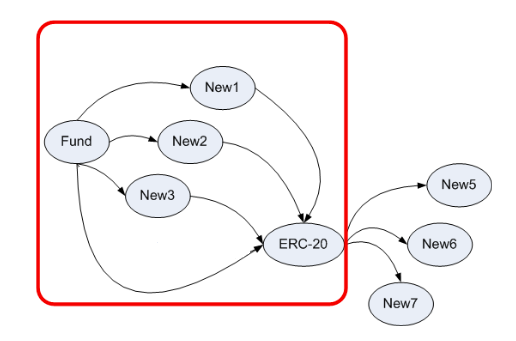
\includegraphics[width=0.6\columnwidth]{images/illustrativeExample.png}
    \caption{\csentence{The illustrative Example}}
    \label{fig:illustrativeExample}
\end{figure}

While the number of accounts in this illustrative example is minimal, the associated figure does illustrate the indicative graph-typology for a pump-and-dump attack: the underpinning, undirected sub-graph of the graph in the enclosed boundary-box. It contains a number of cycles (6 in this case), all with two common nodes: the token and the initial fund account. The paths that make up these undirected cycles can contain zero, one of more intermediate nodes (in this case 0 and 1). Our position is that this topology in the transaction graph is indicative of a pump-and-dump attack. 

%in fact, I find it very tough to equate this with the circled sub-graph in the 'Extracted example-block range from Kovan, partially because there are no edge directions but also because there are no node titles to guide me. I tried to annotate using snagit, and attach the figure (2nd attachment in the email), maybe as an overlay on your current figure 2?

We begin by planting the sample data on the blockchain:
\begin{itemize}
    \item The ERC-20 of CycleToken (CYC) at address \\ {\tiny\texttt{0xED53b...8A0}}
    \item The account, ``fund,'' which will be the main source of funds to fund all transactions at address {\tiny\texttt{0x5c1bb...152}}
    \item The layer of indirection accounts, to hide the activities of the source of funds account at addresses:
    \begin{itemize}
        \item ``new1'' : ``{\tiny\texttt{0xe86c92...380}}''
        \item ``new2'' : ``{\tiny\texttt{0xfcb67f...980}}''
        \item ``new3'' : ``{\tiny\texttt{0xdcb6d4...b6a}}''
    \end{itemize}
    \item And the three further liquidity accounts:
    \begin{itemize}
        \item ``new4'' :``{\tiny\texttt{0xd78112...464}}''
        \item ``new5'' :``{\tiny\texttt{0x1da779...b04}}''
        \item ``new6'' :``{\tiny\texttt{0x4c822b...8dc7}}''
    \end{itemize}
\end{itemize}

Then we executed the set of transactions proposed:
\begin{itemize}
    \item Funding the transaction costs of the dummy accounts by transferring ether to ``new1,'' ``new2'' and ``new3'' from ``fund''
    \item Having ``new1,'' ``new2,'' ``new3'' and ``fund'' purchase tokens by executing ``{\tiny\texttt{transfer()}}'' on the ERC-20.
    \item Further trading those tokens to ``new4,'' ``new5'' and ``new6'' from ``new1,'' ``new2'' and ``new3'' by executing ``{\tiny\texttt{transfer()}}'' on the ERC-20.
\end{itemize}

This activity occurs between blocks {\tiny\texttt{0x7D0090}} and {\tiny\texttt{0x7D01B8}}.  Next, in line with Section \ref{extraction}, we extract the raw blocks from the blockchain.  The main Ethereum node clients, \emph{geth} and \emph{parity}\cite{pustivsek2018approaches} expose a JSON RPC API that can be queried to extract the blocks. For example, to query the first block in our range, {\tiny\texttt{0x7D0090}}, we could issue a ``curl''\cite{powers2003unix} request as follows:

\begin{lstlisting}[basicstyle=\tiny]
    curl 'http://10.41.5.92:8545' -X POST -H "Content-Type: 
    application/json" --data '{"jsonrpc":"2.0","method":
    "eth_getBlockByNumber", "params": ["0x7D0090",true],"id":1}'
\end{lstlisting}

Which results in a JSON\cite{crockford2006application} response detailing the entire block, including a full listing of all the transactions in that block. 

We create the vertices and edges of the graph from the ``to'' and ``from'' fields of this data, being careful not to add any of the vertices or edges that already exist more than once.  This representation is then outputted to a file in graphSON\cite{tomaszuk2016rdf}  format.  Here is an example of a single vertex and its adjacency list in graphSON:

\begin{lstlisting}[basicstyle=\tiny]
{
  "id": { "@type": "g:Int64",  "@value": 1515 },
  "label": "account",
  "inE": {
    "transacts": [ {
        "id": { "@type": "g:Int64", "@value": 4916 },
        "outV": { "@type": "g:Int64", "@value": 1514 }
      } ]
  },
  "properties": {
    "hex": [ { "id": { "@type": "g:Int64", "@value": 4917 },
        "value": "0x02360ed0b4ed60439b
                        1766c66fefaaf598299182"
      } ]
  }
}
\end{lstlisting}

The extracted range of blocks, rendered as a graph is shown in Figure \ref{fig:toyfullgraph}.  Even on the test network you can see a lot of independent activity making a disconnected graph.  Our transactions are circled at the top of the graph.

% Note Andy: this involves my 2nd attachment figure being placed into this fig - Jim


\begin{figure}
    \centering
    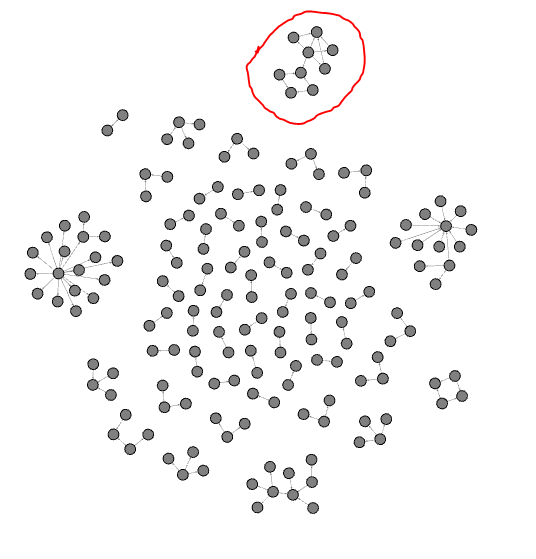
\includegraphics[width=0.6\columnwidth]{images/toy_full_graph.png}
    \caption{Extracted example block range from Kovan.}
    \label{fig:toyfullgraph}
\end{figure}

Next we start our Tinkerpop GraphDB and load the json file with the command:

\begin{lstlisting}[basicstyle=\tiny]
graph.io(IoCore.graphson()).readGraph("D:/graph.json")
\end{lstlisting}

and then run our query, from Section \ref{graphtraversal} to generate the sub graph of cycles, originating with our CycleToken contract.  We can then export the traversal to a graphML file using the command:

\begin{lstlisting}[basicstyle=\tiny]
subg.io(graphml()).writeGraph('D:/graph.graphml')
\end{lstlisting}

Finally, we can load the graphML file in Gephi, which produces the graph in Figure \ref{fig:toygraph}, which we have annotated here for readability.  You can see in the output the bad actors participating in suspicious behaviour; The token, the fund wallet and the indirection wallets used to distribute purchases.  This is further described by the calculated metrics in Table \ref{tab:toystats}.

% I dont see fund wallet having 4 outgoing edges as the example implied??? - Jim

\begin{figure}
    \centering
    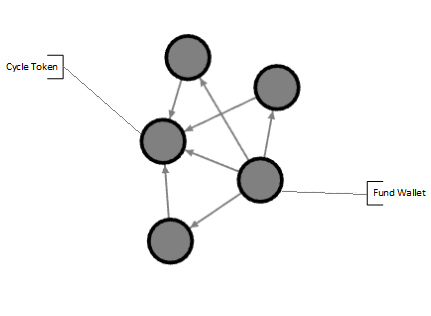
\includegraphics[width=0.5\columnwidth]{images/toy_graph.png}
    \caption{The result of traversal of CycleToken.}
    \label{fig:toygraph}
\end{figure}

\begin{table}[]
    \centering
\begin{tabular}{|l|l|}
\hline
\textbf{Metric}                & \textbf{Value} \\ \hline
Cycle Length             & 3              \\ \hline
Total Transactions             & 4              \\ \hline
Cycles            & 3              \\ \hline
Ancestor Level, $n$            & 1           \\ \hline
Wallets Transferring to ERC-20, $\psi$ & 4              \\ \hline
Wallets Sharing Common Ancestor at $n$, $\tau$            & 3           \\ \hline
Common Ancestors at $n$            & 1           \\ \hline
Funding-Origin Indirection, $\iota$            & 0.75           \\ \hline
\end{tabular}
    \caption{Stats for CycleToken example, with $n=1$.}
    \label{tab:toystats}
\end{table}


\section{Case Study of a Known Attack: iFishYunYu}
During early July of 2018, the gas price\footnote{The price paid to execute a transaction on the Ethereum network.} rose by 500\% to an Ether price of 100GWei\footnote{Wei is the smallest subdivision of Ether at $10^-18$.  GWei or GigaWei or a ``Shannon'' is $10^-9$}.  The price for transactions is market driven.  A submitted transaction states the price the submitter is willing to pay to have her transaction mined. As such, during high volume periods, or periods where a number of willing actors willing to pay a higher gas price submit to the network, the price of gas can rise.  A submitter would often submit a transaction with a high gas price in order to have their transaction mined quicker, which would be especially useful if the value transfer was high or important. The 500\% rise was, however, unprecedented in Ethereum's short history.  On closer inspection of the block range {\tiny\texttt{0x5AC91B}} to {\tiny\texttt{0x5B009B}} where the rise occurred we find over 80,000  transactions centered around a single ERC-20 contract called iFishYunYu \footnote{Contract address \tiny\texttt{0x98b4ca8bd52e4ed1f28d3f30d9f567d1166c9483}}.  These transactions were submitted with gas prices in excess of 147GWei.  Furthermore, while it can validly be argued that no virtual representation of ownership, be it a common security or a blockchain token, has no intrinsic value in an of itself, iFishYunYu did not even purport to represent any real world asset.  Normally an ERC-20 is linked to additional meta-data describing an asset or platform that it represents utility or ownership of.  This meta-data usually includes source code of the contract and links to the real world company presence offering the token. No such supporting documentation existed with iFishYunYu.  Forums, chat groups, blockchain news sites and other accepted primary sources for blockchain community news \cite{li2019cryptocurrency,kamps2018moon} associated with the Ethereum network leveled accusations of attempting to inflate the perceived volumes of the contract to fraudulently gain a listing on token exchanges, or a bad actor deliberately attempting to prove a point on the vulnerability of the Ethereum network \cite{ifishweb1,ifishweb2}.  What is certain that at a high gas price of 147 Gwei, the 80k+ transactions executed amounted to very expensive endeavour totally \$285,000\footnote{Given 52325 gas per transfer, a gas price of 147Gwei and the USD to ETH exchange rate of \$464.13 during the period.} in transaction fees for a token of no obvious representative value. 

Enough circumstantial evidence existed to suspect malicious behaviour and warrant further investigation.  We ran through our process twice, producing results for the presence of 3 and 4 length cycles.  Figure \ref{fig:ifish3hop} shows the graph for cycles of size 3.  A visual inspection allows us to identify the iFish contract and 2 wallets that appear to be acting as a source of funds for other wallets as a layer of indirection between them and the purchase of tokens. There is also a third vertex above and to the left with far few incoming connections that is also 2 hops away from iFish.  The three wallet addresses are:

\begin{itemize}
    \item {\tiny\texttt{0x8c1b1473cffc7ff621c8b50316c90a0b8b32558a}}
    \item {\tiny\texttt{0x91a79c71a702942135814a6746d71f2ef0ae0262}}
    \item {\tiny\texttt{0x45f64a7148d1cfeded427dd4380b458877e7ce56}}
\end{itemize}

\begin{figure}
    \centering
    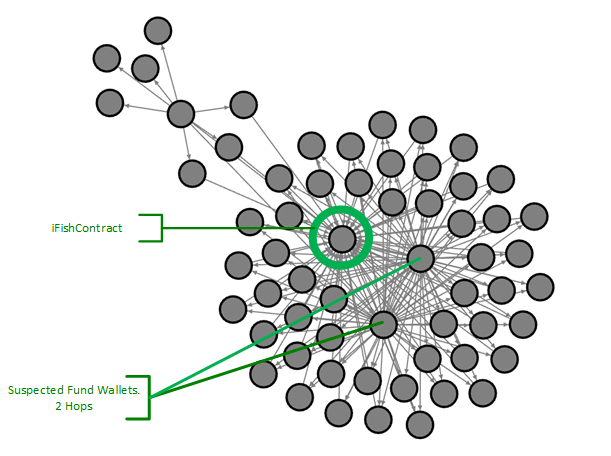
\includegraphics[width=0.8\columnwidth]{images/iFish3hop.png}
    \caption{Sub-graph of cyclic behaviour centered around the iFishYunYu contract with a cycle length of 3.}
    \label{fig:ifish3hop}
\end{figure}

Figure \ref{fig:lifecycle} shows the output where we consider cycles of length 4 on this data-set.   Visually, it becomes immediately obvious that only 5 new wallets (in addition to the previous 3 identified) are the source of the vast majority of transactions:

\begin{itemize}
    \item {\tiny\texttt{0xa9a0f46f8e24a7f9153333b50659a2e7e6875ecc}}
    \item {\tiny\texttt{0xa6d73d0e15f811e6945bc270c5825918da2645b1}}
    \item {\tiny\texttt{0x7c1cff9e521cffba0c45859dbd274982c44c45b3}}
    \item {\tiny\texttt{0x4d1167c167a080d6b973561a3b7683cc998108e1}}
    \item {\tiny\texttt{0xe47093061140f7e2e8b81b78bfc322dc70b50259}}
\end{itemize}

The metric is shown in Table \ref{tab:ifish4hop}. When we examine the metric from Table \ref{tab:ifish4hop} we are drawn to the conclusion that \emph{every} transaction during this time period on the ERC-20 originated in a wallet with a common ancestor of 1 and 2.  A striking attribute of this attack is that every transaction is also involved in a cycle, and highlights the severity and blatant nature of the attack.  We would expect a more subtle combination of normal trading combined with attack originating trades were we to examine other suspicious ERC-20's.
    

\begin{table}[]
    \centering
\begin{tabular}{|l|l|}
\hline
\textbf{Metric}                & \textbf{Value} \\ \hline
Cycle Length             & 4              \\ \hline
Ancestor Levels, $n$            & 1 and 2          \\ \hline
Wallets Transferring to ERC-20, $\psi$ & 1633              \\ \hline
Wallets Sharing Common Ancestor at $n$, $\tau$            & 1630           \\ \hline
Common Ancestors at $n$            & 8           \\ \hline
Funding-Origin Indirection, $\iota$            & 0.998          \\ \hline
\end{tabular}
    \caption{Stats for iFish, with $n=2$.}
    \label{tab:ifish4hop}
\end{table}



\begin{figure}
    \centering
    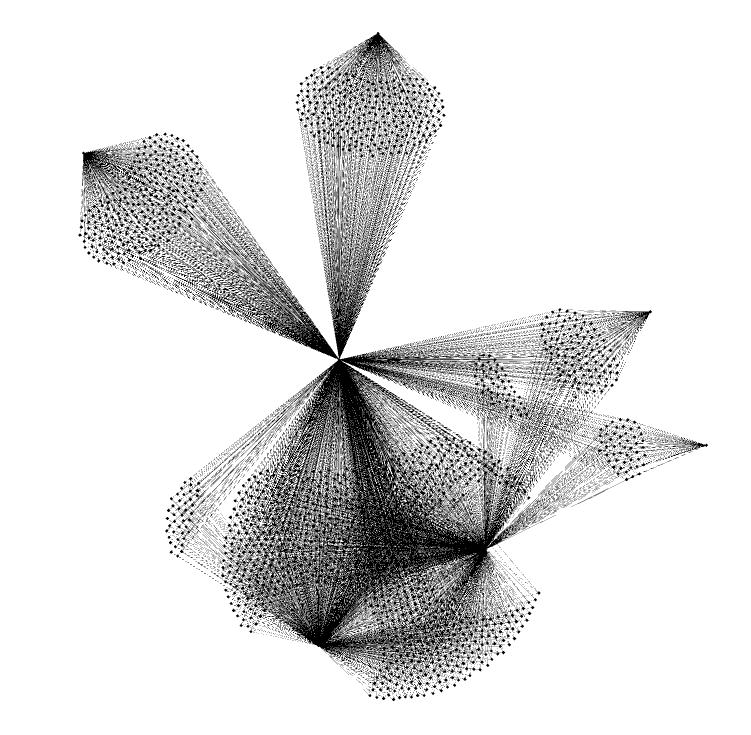
\includegraphics[width=0.8\columnwidth]{images/ifishattack.png}
    \caption{Sub-graph of cyclic behaviour centered around the iFishYunYu contract with a cycle length of 4.}
    \label{fig:lifecycle}
\end{figure}

These results help confirm the suspicions of the community expressed regarding this trading period. If there was even a single purchaser of the token operating as normal we would have expected to see a non cyclic wallet executing a transfer to the contract address and producing a result for $\rho < 1$.

\section{Future Work}
The work presented in this paper can branch in many directions for future research. Adding weighting to the edges based on the count of transactions between vertices rather than collapsing all transactions between two vertices to a single edge could reveal further insights into the data.  Similarly adding meta data to the edges such as the timestamp would also be useful in expanding the analysis.

We are also eager to experiment with other types of graph als applied in software reengineering research to see if they yield similarly useful results in the blockchain space.

The framework can be extended to detect other coordinated financial crimes, including wash trading, rug pulls, and complex money laundering schemes \cite{song2024identifying}.

Future work will integrate our graph-based features with advanced machine learning models, including Graph Neural Networks, to automate the classification of normal versus suspicious patterns. This will incorporate temporal dynamics and edge weighting for detecting more subtle patterns and expanding analysis to multiple tokens and longer historical ranges \cite{Harper2025STGNN, Chen2024Phishing, Sultana2025GNN, song2024identifying}.

The work in this paper focuses on a single known attack. We would like to expand this work to examine a much larger population of past ICOs with the dual goal of benchmarking our metric and possibly to reveal past malicious behaviour on ICOs that had previously been deemed problem free.  Conversely, examining past ICO trading profiles that have no reported suspicious behaviour could be very useful in defining what a ``normal'' trading profile looks like.  For example, in Figure\ref{fig:4icos} we applied the cycle detection algorithm to busy trading periods of the large market capitalized ICO's of Envion, Swissborg, Bancor and Aeternity. The graphs produced are notably different and suggest the distinction between an attack and normal trading can readily be revealed.

\begin{figure}
    \centering
    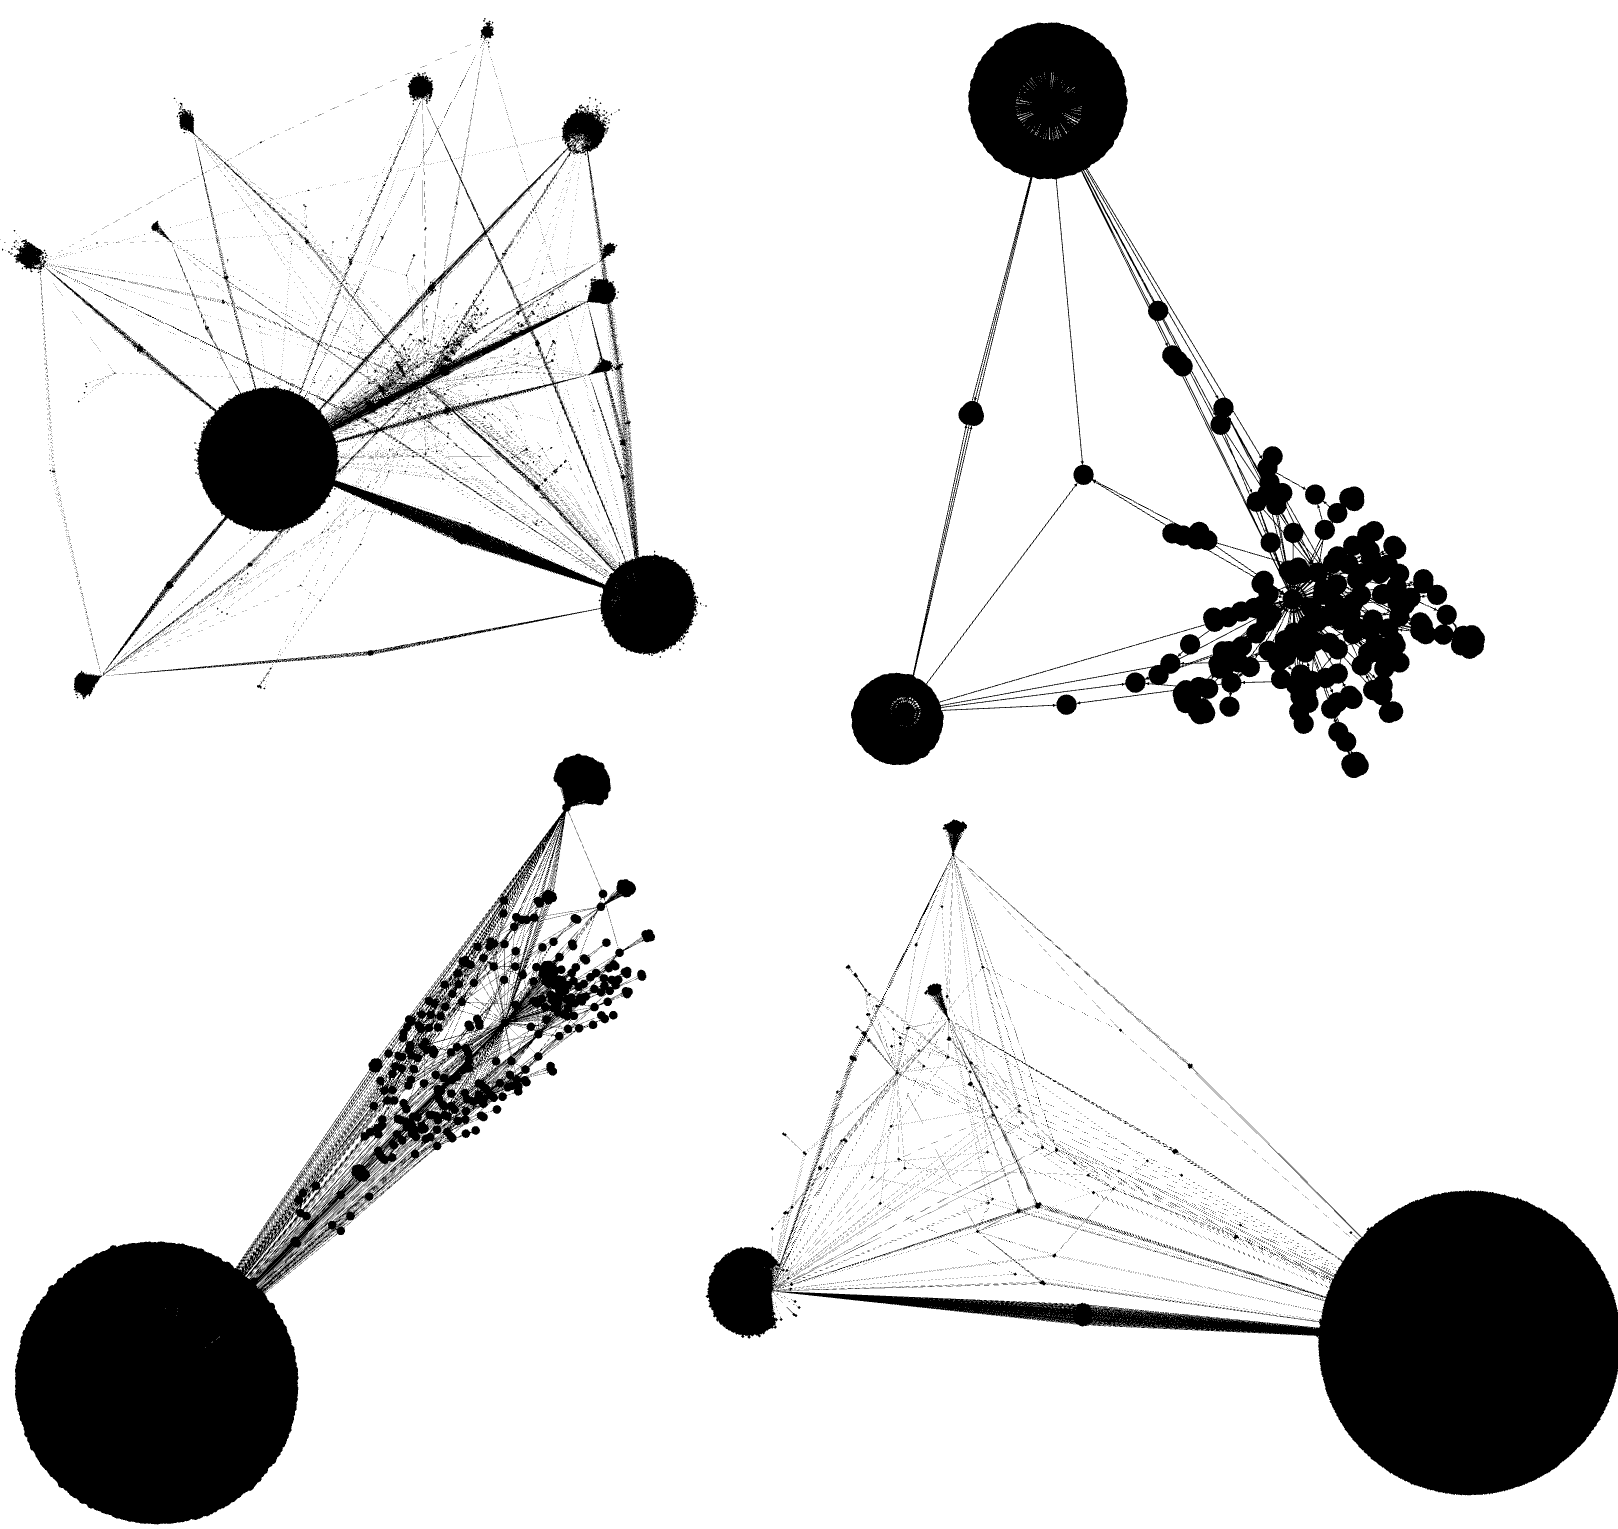
\includegraphics[width=0.5\columnwidth]{images/4icos.png}
    \caption{Sub-graph of cyclic behaviour centered around Envion, Swissborg, Bancor and Aeternity smart contracts with a cycle length of 4.}
    \label{fig:4icos}
\end{figure}


\section{Threats to Validity and Limitations}\label{sec:threats}
This study uses snapshots of the blockchain to focus the analysis to active periods of trading on the ERC-20. While useful in terms of execution time and result size, it is also possible that by excluding data we are missing important information.  

Furthermore, we have deliberately limited the size of analyses to three and four levels of ancestors.  This is in line with what we perceive as an obvious attempt at fraud - i.e. placing a layer of indirection between a source of funds and a purchase.  However, any number of layers of indirection could conceivably be placed between a source of funds and the contract, making this constraint less general a solution.

To gain more confidence in these results we would also propose expanding the number of case studies and interviewing stakeholders in known ICO's to add secondary confirmation of our results and also to report the result of the same approach on other traded tokens.

Also, as implemented here, our analysis tools will not scale to larger snapshots greater than 1 million nodes, on a PC with 4Gb of RAM.  The query would need to be reorganized to take advantage of a ``MapReduce'' implementation as described in Section \ref{graphtraversal} \cite{dean2008mapreduce}.


\section{Conclusion}
Fraud and other malicious behaviour exists and is a real concern on unregulated trading environments hosted on the blockchain.  In this paper we highlight one such approach to game the token market and demonstrate a viable approach, applied to a confirmed positive attack, to revealing this behaviour on other ICO's. Our approach can be refined further in dimensions such as cycle depth, temporality, and edge weighting in the future, as well as interesting comparisons of the cycle profiles against healthy trading. However, as exists in this paper, our approach provides a novel and valuable blockchain forensics approach for regulators and auditors to examine a token offering for suspect behaviour.

\subsection{Acknowledgements}
This research was funded by Science Foundation Ireland under grant number 13/RC/2094 in conjunction with Horizon Globex Ltd. under statement of work SOW2017-055.

\vspace{12pt}

% Bibliography setup
\bibliographystyle{IEEEtran}
\bibliography{IEEEexample}

\end{document}
